\documentclass{article}
\usepackage{amsmath, amssymb, amsthm}
\usepackage{tikz}
\usetikzlibrary{positioning}

\newcommand{\Ac}{\mathcal{A}}  % alphabet
\newcommand{\Lc}{\mathcal{L}}  % label function
\newcommand{\Gc}{\mathcal{G}}  % labeled graph
\newcommand{\Hc}{\mathcal{H}}  % labeled graph
\newcommand{\Vc}{\mathcal{V}}
\newcommand{\Ec}{\mathcal{E}}
\newcommand{\Bc}{\mathcal{B}}
\newcommand{\Kc}{\mathcal{K}}
\newcommand{\Fc}{\mathcal{F}}
\newcommand{\shift}[1]{\mathsf{X}_{#1}}
\newcommand{\term}[1]{\textit{#1}}
\newcommand{\Sync}{\textsf{Sync}}

\theoremstyle{definition}
\newtheorem{theorem}{Theorem}
\newtheorem{definition}{Definition}
\newtheorem{lemma}{Lemma}

\renewcommand{\baselinestretch}{1.15}
\setlength{\parskip}{.05em}

\begin{document}

\section{Preliminaries}

\begin{definition}
    Let \(\Ac\) be a finite set. The \term{full \(\Ac\)-shift} is the set \(\Ac^\mathbb{Z}\) of all 
    bi-infinite sequences over \(\Ac\) (i.e. functions from \(\mathbb{Z}\) to \(\Ac\), hence the 
    usual notation for the set of all functions from \(\mathbb{Z}\) to \(\Ac\)).
\end{definition}

\noindent A \term{block} (or \term{word}) is a finite sequence of letters over some alphabet \(\Ac\). 
Let \(x=(x_i)_{i \in \mathbb{Z}}\) be a bi-infinite sequence. For \(i \leq j\), the block from the 
\(i\)th coordinate to the \(j\)th coordinate is denoted \[x_{[i,j]} \triangleq x_i x_{i+1} \dots x_{j}.\]

\begin{definition}
    Let \(\Fc\) be a set of words over some alphabet. A \term{subshift} is a subset \(\shift{\Fc}\)
    of some full shift \(\Ac^\mathbb{Z}\) such that no word in \(\Fc\) appears in any point of the subshift,
    defined as
    \[\shift{\Fc} \triangleq \Big\{ \; (x_i)_{i \in \mathbb{Z}} \in \Ac^\mathbb{Z} \; : \; \forall i, j \in \mathbb{Z}, i\leq j \quad  x_{[i,j]} \notin \Fc \; \Big\}.\]
\end{definition}

\begin{definition}
    A \term{graph} \(G\) is a \(4\)-tuple \(G = (\Vc, \Ec, i, t)\), where \(\Vc\) is a finite 
    set of \term{vertices}, \(\Ec\) is a finite set of \term{edges}, and \(i : \Ec \to \Vc\) and 
    \(t : \Ec \to \Vc\) are functions assigning an \term{initial} and \term{terminating} vertex for 
    each edge, respectivley. For an arbitrary graph \(G\), let 
    \(\Vc_G\), \(\Ec_G\), \(i_G\), and \(t_G\) denote the graph's vertices, edges, and 
    intial and terminating vertex functions, respectivley. If the choice 
    of \(G\) is understood, then the subscripts will be dropped for notational convenience.

    For \(I \in \Vc\), the \term{outgoing edges of \(I\)} is the set of edges starting at \(I\),
    denoted 
    \[i^{-1}(I) = \{e \in \Ec : i(e) = I\}.\]
    Similary, the \term{incoming edges of \(I\)} is the set of edges terminating at \(I\), 
    denoted
    \[t^{-1}(I) = \{e \in \Ec : t(e) = I\}.\]

    A graph is \term{essential} if all verticies have at least one incoming and outgoing edge;
    i.e. for all \(I \in \Vc\), \(i^{-1}(I) \ne \varnothing\) and \(t^{-1}(I) \ne \varnothing\).

\end{definition}

\begin{definition}
    A \term{labeled graph} \(\Gc\) is a pair \(\Gc = (G, \Lc)\), where \(G\) is a graph and \(\Lc : \Ec \to \Ac\) is the 
    \term{labeling function} from the edges of \(G\) onto some finite alphabet \(\Ac\).

    A labeled graph is \term{deterministic} if for each vertex, the labels of the outgoing edges at that vertex are all distinct 
    (i.e. \(\Lc|_{i^{-1}(I)}\) is injective for all \(I \in \Vc\)).
\end{definition}

\begin{definition}
    Let \(G\) be a graph. The \term{edge shift of \(G\)} is the set \(\shift{\Gc}\) of all bi-infinite 
    paths on \(G\), defined as 
    \[\shift{G} \triangleq \Big\{ \; (x_i)_{i \in \mathbb{Z}} \in \Ec^\mathbb{Z} \; : \; \forall i \in \mathbb{Z} \quad t(x_i) = i(x_{i+1}) \; \Big\}. \]
\end{definition}

\noindent As a consequence of this definintion, \(\Bc(\shift{G})\) is the 
set of all finite paths on \(G\), so elements of \(\Bc(\shift{G})\) are called
\term{paths on \(G\)}.


\begin{definition}
    Let \(\Gc = (G, \Lc)\) be a labeled graph. The \term{presentation of \(\Gc\)} is the set \(\shift{\Gc}\)
    of the labels of all bi-infinite paths from \(\shift{G}\), defined as the image of 
    \(\Lc_\infty\) under \(\shift{G}\): \[\shift{\Gc} \triangleq \Lc_\infty(\shift{G}).\]
    We say a word \(w \in \Bc(\shift{\Gc})\) is \term{presented by a path} \(\pi \in \Bc(\shift{G})\) if \(\Lc(\pi) = w\).
\end{definition}

\begin{definition}
    Let \(\Gc = (G, \Lc)\) be a labeled graph. 
\end{definition}

    


\section{Irreducibility}

\noindent Consider the graph \(\Gc\):

\begin{figure}[h]
    \centering
    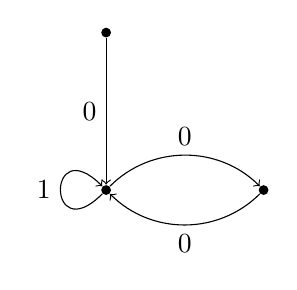
\begin{tikzpicture}
        [vertex/.style={circle, radius=10mm, fill=black, inner sep=1.25pt}]
        \node[vertex] (A) at (0,0) {};
        \node[vertex] (B) at (2,0) {};
        \node[vertex] (C) at (0,2) {};

        \path [->] (A) edge[out=225, in=135, distance=10mm] node[left] {$1$} (A);
        \path [->] (A) edge[out=45, in=135] node[above] {$0$} (B);
        \path [->] (B) edge[out=225, in=-45] node[below] {$0$} (A);
        \path [->] (C) edge[out=270, in=90, distance=2mm] node[left] {$0$} (A);
    \end{tikzpicture} 
\end{figure}




\begin{theorem}
    If \(v \in \Vc_\Hc\), then \(v\) is synchronizing for \(\Gc\Hc\).
\end{theorem}

\begin{proof}
    For any word \(w \in \Bc(\shift{\Hc})\), Let
\end{proof}

\begin{theorem}
    If \(\shift{\Gc\Hc}\) is irreducible, then \(\shift{\Gc} \subseteq \shift{\Hc}\).
\end{theorem}

\begin{proof}
    Let \(\Lc(\pi) \in \Bc(\shift{\Gc})\). As \(\Gc\) is strongly connected,
    there is a path \(\tau \in \Bc(\shift{G})\) with \(t(\tau) = J\) and \(\pi\tau \in \Bc(\shift{G})\).
    Hence, the word \(\Lc(\pi\tau e) = w\) 
\end{proof}

    \begin{theorem}
        If \(\mathcal{G} = (G, \mathcal{L})\) is the minimizing right resolving
        presentation of an irreducible sofic shift \(X\) and \(X\) is and
        \(N\)-step shift of finite type, then \(\shift{G} \cong \shift{\Gc}\).
    \end{theorem}
    
    \begin{proof}
        Let \(x, y\) be walks in \(\shift{G}\). Suppose \(\mathcal{L}_\infty(x)=\mathcal{L}_\infty(y)\),
        For any \(i\), the paths \(x_{[i-N, i-1]}\) and \(y_{[i-N, i-1]}\) present 
        the same word. Because that word is of length \(N\), the word is synchronizing
        for \(\mathcal{G}\) (from 3.4.17), so those paths end at the same vertex. Since
        \(\mathcal{L}(x_{[i]}) = \mathcal{L}(y_{[i]})\), \(\mathcal{G}\) is right 
        resolving, and \(x_{[i-N, i-1]}\) and \(y_{[i-N, i-1]}\) end at the same vertex,
        then \(x_{[i]} = y_{[i]}\) and hence \(x = y\), so \(\mathcal{L}_\infty\) is injective.
        By definition, \(\mathcal{L}_\infty\) is surjective. Therefore, \(\mathcal{L}_\infty\) is bijective and 
        a conjugacy from \(\mathsf{X}_G\) to \(\mathsf{X}_\mathcal{G}\).
    \end{proof}



    % \begin{definition}
    %     Let \(G\) and \(H\) be graphs. A \term{graph homomorphism from \(G\) to \(H\)} is 
    %     a pair \((\partial\Phi, \Phi)\) where \(\partial\Phi: \Vc_G \to \Vc_H\) 
    %     maps verticies of \(G\) to verticies of \(H\) and \(\Phi: \Ec_G \to \Ec_H\) maps 
    %     edges of \(G\) to edges of \(H\),
    %     such that \(\partial\Phi(i_G(e)) = i_H(\Phi(e))\) 
    %     and \(\partial\Phi(t_G(e)) = t_H(\Phi(e))\)
    %     for all edges \(e \in \Ec_G\). 

    %     If both \(\partial\Phi\) and \(\Phi\) are bijective, then the pair is called 
    %     a graph isomorphism between \(G\) and \(H\). The two graphs are graph isomorphic (or simply isomorphic) 
    %     if there exists a graph isomorphism between them, and is denoted \(G \cong H\).
    % \end{definition}

    % \begin{definition}
    %     A \term{labeled graph} is a pair \((G, \Lc)\)
    % \end{definition}

    % \begin{lemma}
    %     Let \(G\) and \(H\) be graphs, and \((\partial\Phi, \Phi)\) be a graph isomorphism 
    %     between them. Then the inverse pair of maps \((\partial\Phi^{-1}, \Phi^{-1})\) is 
    %     a graph homomorphism from \(H\) to \(G\).
    % \end{lemma}

    % \begin{proof}
    %     For an edge \(e_G \in \Ec(G)\), we have 
    %     \begin{align*}
    %         \partial\Phi(i(e)) &= i(\Phi(e))  \\
    %         \partial\Phi^{-1}(\partial\Phi(i(e))) &= \partial\Phi^{-1}(i(\Phi(e)))\\
    %         i(e) &= \partial\Phi^{-1}(i(\Phi(e)))
    %     \end{align*}
    %     Hence, for an edge \(e_H \in \Ec(H)\), \(\Phi^{-1}(e_H) \in \Ec(G)\) so 
    %     \begin{align*}
    %         i(\Phi^{-1}(e_H)) &= \partial\Phi^{-1}(i(\Phi(\Phi^{-1}(e_H))))\\
    %         &= \partial\Phi^{-1}(i(e_H))
    %     \end{align*}
    %     A similar argument shows that \(t(\Phi^{-1}(e_H)) = \partial\Phi^{-1}(t(e))\).
    % \end{proof}

    % \begin{definition}
        
    % \end{definition}

    % \begin{definition}
    %     Let \(\Gc = (G, \Lc_G)\) and \(\Hc = (H, \Lc_H)\) be labeled graphs.
    %     A label-graph isomorphism is a graph isomorphism \((\partial \Phi, \Phi) : G \to H\)
    %     such that \(\Lc_H(\Phi(e)) = \Lc_G(e)\) for all \(e \in \Ec(G)\), which is 
    %     denoted \((\partial \Phi, \Phi) : \Gc \to \Hc\). If there exists a label-graph 
    %     isomorphism between \(\Gc\) and \(\Hc\), then \(\Gc\) and \(\Hc\) are label-graph
    %     isomorphic (or just isomorphic) and is denoted \(\Gc \cong \Hc\).
    % \end{definition}       

    % \begin{theorem}
    %     Let \(\Gc = (G, \Lc_G)\) and \(\Hc = (H, \Lc_H)\) be labeled graphs. 
    %     If \(\Gc \cong \Hc\), then \(\shift{\Gc} = \shift{\Hc}\).
    % \end{theorem}

    % \begin{proof}
    %     For \(x \in \shift{\Gc}\), there exists a \(y \in \shift{G}\) such that \(x_i = \Lc_G(y_i) = \Lc_H(\Phi(y_i))\).
    %     Note that for all \(i \in \mathbb{Z}\),
    %     \begin{align*}
    %         t(y_i) &= i(y_{i+1})\\
    %         \partial \Phi(t(y_i)) &= \partial\Phi(i(y_{i+1}))\\
    %         t(\Phi(y_i)) &= i(\Phi(y_{i+1}))
    %     \end{align*}
    %     so \(\Phi_\infty(y) \in \shift{H}\) and therefore \(x=\left( \Lc_H \circ \Phi \right)_\infty(y) \in \shift{\Hc}\).
    % \end{proof}

    \begin{lemma}
        If \(X\) and \(Y\) are shift spaces, then \(\Bc(X) \subseteq \Bc(Y)\) if and only if \(X \subseteq Y\).
    \end{lemma}

    \begin{proof}
        Let \(x\) be a point in \(X\). Then every word that appears in \(x\) is in \(\Bc(X)\). Since 
        \(\Bc(X) \subseteq \Bc(Y)\), then every word that appears in \(x\) is in \(\Bc(Y)\),
        so \(x \in Y\), hence \(X \subseteq Y\).

        Conversely, let \(w\) be a word in \(\Bc(X)\). Then \(w\) occurs in some \(x \in X\). 
        Since \(X \subseteq Y\), we have \(x \in Y\), so \(w\) occurs in some \(x \in Y\). Hence, \(w \in \Bc(Y)\).
    \end{proof}

    Let \(\Gc\) and \(\Hc\) be labeled graphs, \(I\) be a vertex from \(\Gc\), and \(J\) 
    be a vertex from \(\Hc\). Define the \term{graph connecting \(\Gc\) to \(\Hc\) via \(I\) and \(J\)} 
    as the disjoint union of the two graphs, adding an edge starting at \(I\) and ending at \(J\), 
    and adding a self loop on \(J\). Label these two new edges with a symbol that 
    does not appear in either graph. 
    Since \(\Gc\) and \(\Hc\) are subgraphs of a graph connecting the two,
    it follows that the presentations of the individual graphs are subshifts of a presentation 
    of a graph connecting the two - any bi-infinite walk in one of the graphs is a x
    bi-infinite walk of the corresponding subgraph of the connected graphs.
    Additionally, observe that the graph is reducible,
    as any path starting in \(\Hc\) cannot end in \(\Gc\).
    

    \begin{figure}[ht]
        \centering
        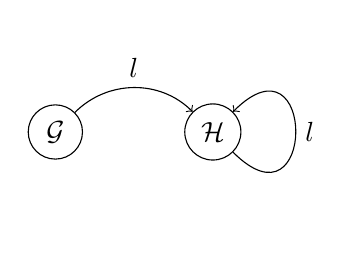
\begin{tikzpicture}
            \node[shape=circle, draw=black] (G) at (0,0) {\(\Gc\)};
            \node[shape=circle, draw=black] (H) at (2,0) {\(\Hc\)};
    
            \path [->] (G) edge[out=45, in=135] node[above] {\(l\)} (H);
            \path [->] (H) edge[out=-45, in=45, distance=15mm] node[right] {\(l\)} (H);
    
        \end{tikzpicture} 

        \caption{A graph connecting \(\Gc\) to \(\Hc\).}
    \end{figure}

    \begin{theorem}
        Let \(\Gc\) and \(\Hc\) be irreducible graphs, and \(\Kc\) be the graph connecting 
        \(\Gc\) to \(\Hc\) via \(I\) and \(J\).
        If \(\shift{\Kc}\) is irreducible, then
        \(\shift{\Gc} \subseteq \shift{\Hc}\).
    \end{theorem}

    \begin{proof}
        First, suppose that \(\shift{\Kc}\) is irreducible, and let \(u \in \Bc(\shift{\Gc})\). 
        There is a path in \(\Gc\) that presents \(u\), hence there is a path in the 
        \(\Gc\) subgraph of \(\Kc\) that presents \(u\). From the irreducibility of 
        \(\Gc\), there is a path from the terminating vertex of a path presenting 
        \(u\) to \(I\). Let \(v\) be the word such path presents and \(l\) be 
        the label of the edge connecting \(\Gc\) to \(\Hc\), so that we have 
        \(uvl \in \Bc(\shift{\Kc})\) and \(u \in \Bc(\shift{\Kc})\). As \(\shift{\Kc}\)
        is irreducible, there exists a word \(w \in \Bc(\shift{\Kc})\) such that 
        \(uvlwu \in \Bc(\shift{\Kc})\). A path presenting \(uvlwu\) must have the 
        subpath presenting \(wu\) visit verticies only from the \(\Hc\) subgraph of \(\Kc\).
        This implies that there is a path in \(\Hc\) presenting \(u\), so we have 
        \(u \in \Bc(\shift{\Hc})\) and therefore \(\Bc(\shift{\Gc}) \subseteq \Bc(\shift{\Hc})\),
        and \(\shift{\Gc} \subseteq \shift{\Hc}\) via Lemma 1.
        % Consider two words \(u, v\) from \(\Bc(\shift{\Kc})\). Suppose there is a path 
        % that presents \(u\) and ends in \(\Gc\) and a path \(\)
        %
        % Then there is always a word \(w \in \Bc(\shift{\Kc})\)
        % such that \(uwv \in \Bc(\shift{\Kc})\), as from 
        %
        % Conversely, suppose \(\shift{\Gc} \subseteq \shift{\Hc}\). Let \(u, v\) be words from \(\Bc(\shift{\Kc})\),
        % and \(\pi, \tau\) be paths presenting \(u\) and \(v\), respectivley. 
        % If \(\pi\) ends in \(\Gc\), then consider either the case where \(\tau\) starts 
        % in \(\Gc\) and the case where \(\tau\) starts in \(\Hc\).
        % In the first case, from irreducibility of \(\Gc\), there is a path 
        % connecting \(\pi\) to \(\tau\). In the second case, from the irreducibility 
        % of \(\Gc\), there is a path connecting \(\pi\) to the path starting at \(I\) and 
        % ending at \(J\) (that is, the edge connecting \(\Gc\) to \(\Hc\)). From the 
        % irreducibility of \(\Hc\), there is a path from \(J\) to the starting vertex 
        % of \(\tau\), so if \(\tau\) ends in \(\Hc\), then there is a path connecting 
        % \(\pi\) to \(\tau\). Hence, for a word \(u\) with a path ending in \(\Gc\) 
        % that presents it, then there exists a word \(w \in \Bc(\shift{\Kc})\) such 
        % that \(uwv \in \Bc(\shift{\Kc})\).
        % If \(\pi\) does not end in \(\Gc\), then it ends in \(\Hc\). From the 
        % irreducibility of \(\Hc\), there is a path connecting \(\pi\) to \(\tau\)
        % if \(\tau\) starts in \(\Hc\). If \(\tau\) started in \(\Gc\), then there is no
        % path connecting them. However, if \(\tau\) ends in \(\Hc\), then the \(\tau = \tau_1 e \tau_2\)
        % where \(\tau_1\) is a path in \(\Gc\) ending at \(I\).
        % We have \(\Lc(\tau_1) \in \Bc(\shift{\Gc})\) and hence \(\Lc(\tau_1) \in \Bc(\shift{\Hc})\)
        % since \(\shift{\Gc} \subseteq \shift{\Hc}\).
        % This means there is a path \(\tau_1'\) in \(\Hc\) that presents 
    \end{proof}

    \begin{theorem}
        Let \(\Gc\) and \(\Hc\) be irreducible, minimal, right-resolving presentations. 
        If \(\shift{\Gc} = \shift{\Hc}\), then there exists a pair
        of verticies \((I, J) \in (\Vc_\Gc \times \Vc_\Hc)\) such that both the graph connecting \(\Gc\) to \(\Hc\) via 
        \(I\) and \(J\) and the graph connecting \(\Hc\) to \(\Gc\) via \(J\) and \(I\) both 
        present irreducible shifts.

        Equivalently, if for every pair of verticies \((I, J) \in (\Vc_\Gc, \Vc_\Hc)\) 
        the graph connecting \(\Gc\) to \(\Hc\) via \(I\) and \(J\) 
        and the graph connecting \(\Hc\) to \(\Gc\) via \(J\) and \(I\)
        do not both present irreducible shifts.
    \end{theorem}

    \begin{proof}
        Suppose \(\shift{\Gc} = \shift{\Hc}\). Since \(\Gc\) and \(\Hc\) are irreducible,
        minimal, right-resolving presentations of the same shift, they must be 
        isomorphic. Let \((\partial\Phi, \Phi)\) be a graph isomorphism between them. 
        Choose an arbitrary vertex I from \(\Gc\), and then let \(\Kc\) 
        be the graph connecting \(\Gc\) to \(\Hc\) via \(I\) and \(\partial\Phi(I)\).
        Let \(f\) be the self loop on \(\partial\Phi(I)\) added in the construction of
        \(\Kc\), and \(\Hc^+\) be the \(\Hc\) of \(\Kc\) subgraph plus \(f\).
         As 
        \(\Hc\) is irreducible, then \(\Hc^+\) is irreducible. 
        It suffices to show that \(\shift{\Kc} = \shift{\Hc^+}\) to show \(\shift{\Kc}\) 
        is irreducible. 

        % Let \(u, v\) be words from \(\Bc(\shift{\Kc})\),
        % and \(\pi, \tau\) be paths presenting \(u\) and \(v\), respectivley. 
        % If \(\pi\) ends in \(\Gc\), then consider either the case where \(\tau\) starts 
        % in \(\Gc\) and the case where \(\tau\) starts in \(\Hc\).
        % In the first case, from irreducibility of \(\Gc\), there is a path 
        % connecting \(\pi\) to \(\tau\). In the second case, from the irreducibility 
        % of \(\Gc\), there is a path connecting \(\pi\) to the path starting at \(I\) and 
        % ending at \(J\) (that is, the edge connecting \(\Gc\) to \(\Hc\)). From the 
        % irreducibility of \(\Hc\), there is a path from \(J\) to the starting vertex 
        % of \(\tau\), so in total, if \(\tau\) ends in \(\Hc\), then there is a path connecting 
        % \(\pi\) to \(\tau\). Hence, for a word \(u\) with a path ending in \(\Gc\) 
        % that presents it, then there exists a word \(w \in \Bc(\shift{\Kc})\) such 
        % that \(uwv \in \Bc(\shift{\Kc})\).

        % If \(\pi\) does not end in \(\Gc\), then it ends in \(\Hc\). From the 
        % irreducibility of \(\Hc\), there is a path connecting \(\pi\) to \(\tau\)
        % if \(\tau\) starts in \(\Hc\). If \(\tau\) started in \(\Gc\), then there is no
        % path connecting \(\pi\) to \(\tau\). However, if \(\tau\) ends in \(\Hc\), then the \(\tau = \tau_1 e \tau_2\)
        % where \(\tau_1\) is a path in \(\Gc\) ending at \(I\), \(e\) is the edge connecting 
        % \(\Gc\) and \(\Hc\), and \(\tau_2\) is a path in \(\Hc\) starting at \(J\).

        Let \(u\) be a word from \(\Bc(\shift{\Kc})\), and \(\pi\) be a path that presents it.
        Without loss of generality, assume \(u\) and \(\pi\) are nonempty.
        If \(\pi\) starts in \(\Hc^+\), then \(u \in \Bc(\shift{\Hc^+})\). Otherwise, it 
        starts in \(\Gc\) and either ends in \(\Gc\) or ends in \(\Hc^+\). 
        For the case of \(\pi\) ending in \(\Gc\), then \(\Phi(\pi)\) is a path in 
        \(\Hc\) presenting \(u\), as \((\partial\Phi, \Phi)\) is a graph isomorphism,
        so \(u \in \Bc(\shift{\Hc^+})\).
        For the case of \(\pi\) ending in \(\Hc^+\), we can split 
        \(\pi\) into \(\pi=\pi_1 e \pi_2\), where \(\pi_1\) and \(\pi_2\)
        are (possibly empty) paths from \(\Gc\) and \(\Hc^+\), respectivley, and 
        \(e\) is the edge connecting \(\Gc\) and \(\Hc\). Note 
        that \(\Phi(\pi_0)\) is a path in \(\Hc\) and that it terminates
        at \(\partial\Phi(I)\) as \(\pi_0\) terminates at \(I\), assuming \(\pi_0\) is nonempty.
        From this, we have that \(\Phi(\pi_0)f\pi_1\) is path in \(\Hc^+\) that presents \(u\), 
        so \(u \in \Bc(\shift{\Hc^+})\).

        Hence, we have \(\Bc(\shift{\Kc}) \subseteq \Bc(\shift{\Hc^+})\), and from 
        the construction of \(\Kc\), we also have \(\Bc(\shift{\Hc^+}) \subseteq \Bc(\shift{\Kc})\), 
        so \(\Bc(\shift{\Kc}) = \Bc(\shift{\Hc^+})\) and \(\shift{\Kc} = \shift{\Hc^+}\). Thus,
        we have shown the graph connecting \(\Gc\) to \(\Hc\) via \(I\) and \(\partial\Phi(I)\)
        presents an irreducible shift. A similar argument can be made showing that 
        the graph connecting \(\Hc\) to \(\Gc\) via \(\partial\Phi(I)\) and \(I\) presents 
        an irreducible shift (start from ``\dots and then let \(\Kc\)'', and replace
        \(\Gc \mapsto \Hc, \Hc \mapsto \Gc, I \mapsto \partial\Phi(I), \partial\Phi(I) \mapsto I,
        \Hc^+ \mapsto \Gc^+, \Phi(\pi_0) \mapsto \Phi^{-1}(\pi_0)\)).
    \end{proof}

    \begin{theorem}
        Given an oracle for minimizing a reducible presentation, deciding 
        if two irreducible, minimal, right-resolving labeled graphs are isomorphic can be determined in polynomial time.
    \end{theorem}

    \begin{proof}
        Let the decision procedure be as follows:
        for every pair of vertices
        \((I, J) \in (\Vc_\Gc \times \Vc_\Hc)\) between the graphs,
        construct and set \(\Gc_I\to\Hc_J\) as the graph connecting \(\Gc\) to \(\Hc\)
        via \(I\) and \(J\), and similarly, construct and set \(\Hc_J \to \Gc_I\) as the graph connecting 
        \(\Hc\) to \(\Gc\) via \(J\) and \(I\). Then,
        using the oracle, minimize \(\Gc_I \to \Hc_J\) and check if it is strongly connected (that is, irreducible),
        and if so, then from Theorem 2, we know we can 
        set \(\shift{\Gc} \subseteq \shift{\Hc}\) to be true.
        Similary, minimize \(\Hc_J \to \Gc_I\) and check if it is strongly connected, and 
        if so, set \(\shift{\Hc} \subseteq \shift{\Gc}\) to be true.
        If at any point both \(\shift{\Gc} \subseteq \shift{\Hc}\) and \(\shift{\Hc} \subseteq \shift{\Gc}\)
        are set to true, then \(\shift{\Gc} = \shift{\Hc}\) and thus can conclude \(\Gc \cong \Hc\) (as 
        \(\Gc\) and \(\Hc\) are unique, minimal, and irreducible presentations). If you find that 
        after every pair of verticies that one or both  
        of \(\shift{\Gc} \subseteq \shift{\Hc}\) and \(\shift{\Hc} \subseteq \shift{\Gc}\)
        were not set to true, then we have that for all pairs of verticies,
        the presentations of the pair of graphs constructed were not both 
        irreducible, as if they were, then both \(\shift{\Gc} \subseteq \shift{\Hc}\)
        and \(\shift{\Hc} \subseteq \shift{\Gc}\) would be true, so via Theorem 3, we have that \(\shift{\Gc} \neq \shift{\Hc}\)
        and can conclude \(\Gc \ncong \Hc\) (as again, \(\Gc\) and \(\Hc\) are irreducible, minimal, right-resolving 
        graphs).
        
        The worst case runtime of the decision procedure is if \(\Gc \ncong \Hc\),
        as we minimize and check strongly connected-ness twice 
        (of a graph that is potentially the size of both \(\Gc\) and \(\Hc\))
        for each pair of verticies, so the runtime is \(O((V+E)\cdot V^2)\),
        where \(V\) is the number of verticies of one graph and \(E\)
        is the number of edges of one graph.
    \end{proof}
\end{document}